% lutorch_ex library report.
% Build: latexmk -pdf -interaction=nonstopmode -halt-on-error lutorch_ex_report.tex
% fig_curves.pdf (Figure 3) and the benchmark data were produced on branch feature/lutorch_ex_report,
% doc/research/lutorch_ex_report/ (make_fig_curves.py, bench_report.py); the code is src/spiky/lutorch_ex/.
\documentclass[11pt]{article}
\usepackage[margin=1in]{geometry}
\usepackage{lmodern}
\usepackage[T1]{fontenc}
\usepackage{amsmath,amssymb}
\usepackage{booktabs,array,tabularx}
\usepackage{xcolor}
\usepackage{listings}
\usepackage{graphicx}
\usepackage{caption}
\usepackage{tikz}
\usetikzlibrary{positioning,arrows.meta,backgrounds,fit,calc}
\usepackage[numbers]{natbib}
\usepackage{hyperref}
\hypersetup{colorlinks=true,linkcolor=black,citecolor=blue!60!black,urlcolor=blue!60!black,
  pdftitle={The lutorch\_ex library},pdfauthor={Anatoly Starostin}}
\captionsetup{font=small,labelfont=bf,skip=4pt}
\setlength{\parskip}{0.25em}
% typewriter with a line-break opportunity after every underscore and slash (long class and file names)
\DeclareRobustCommand{\code}[1]{{\renewcommand{\_}{\textunderscore\allowbreak}\texttt{#1}}}
\newcommand{\sgn}{\operatorname{sgn}}
\lstset{basicstyle=\ttfamily\footnotesize,columns=fullflexible,breaklines=true,frame=single,language=Python,
        keywordstyle=\color{blue!60!black},commentstyle=\color{green!40!black},showstringspaces=false,
        aboveskip=4pt,belowskip=4pt,xleftmargin=2pt}
\title{\textbf{The \code{lutorch\_ex} library}\\[2pt]\large lookup-table layers: tables, projections, cartridges, and results}
\author{Anatoly Starostin\\DeepSpike Inc.}
\date{October 2026}
\begin{document}
\maketitle
\vspace{-1.2em}

\noindent\textbf{In one paragraph.} \code{lutorch\_ex} is a small PyTorch library of \emph{lookup-table
layers}: drop-in replacements for a feed-forward layer that, instead of multiplying the input by weight
matrices, turn it into a few sign bits, use those bits as addresses into many small learnable tables, and
add up the rows they read. This report walks through it in four parts: how a table is addressed and read,
and how tables form a layer (\S\ref{sec:idea}); a projection wrapper that gives a stack of tables an ordinary vector-in, vector-out
interface, so it can sit anywhere a feed-forward layer would (\S\ref{sec:projection}); \emph{cartridges}
--- interchangeable read mathematics behind
one fixed contract, in three generations, one of which is quantised to int8 and ships with a deployment
path (\S\ref{sec:cartridges}); and the two regularisers every cartridge shares (\S\ref{sec:reg}).
\S\ref{sec:ml} reports a seven-configuration sweep at 48k steps.

% ======================================================================================================
\section{The idea: tables addressed by an LSH}
\label{sec:idea}

A lookup table (LUT) replaces a multiply-accumulate with an \emph{address} and a \emph{read}. Hash the
input to a small integer with a locality-sensitive hash (LSH) --- here, a handful of sign bits --- and
fetch the stored vector at that address. The construction comes from Izhikevich's \emph{Spiking
Manifesto}~\citep{manifesto}: a spiking network stores a vast number of synapses but touches only those of
the neurons that fired, which is exactly what a table read does, and the \emph{order} of spikes rather than
their magnitude carries the information, which is exactly what a sign-bit address encodes.

\paragraph{One table.} Work in a space $z\in\mathbb{R}^{d_\text{in}}$ (Figure~\ref{fig:table}). An
\emph{anchor} is an index into $z$. A table owns \code{nap}\footnote{\code{nap}: the number of anchor
probes per table.} \emph{probes}; probe $j$ is either an anchor
pair $(a_j,b_j)$, giving $u_j=z[a_j]-z[b_j]$, or a single anchor $a_j$, giving $u_j=z[a_j]$. Each probe
contributes one bit $[\,u_j>0\,]$, so an address $c\in[0,K)$ has \code{nap} bits and the table has
$K=2^{\text{nap}}$ cells, each holding a learnable row $W[c]\in\mathbb{R}^{d_\text{out}}$. The magnitudes $|u_j|$ are the
\emph{margins}: how far each bit is from flipping. The smallest one, $u^\star=\min_j|u_j|$, marks the
least certain bit, and flipping that bit gives the \emph{neighbour} cell $c'$ --- the one the input would
land in under the smallest perturbation. Every read mathematics in this library --- every
\emph{cartridge}, in the vocabulary of \S\ref{sec:cartridges} --- uses $c$, $u$, and $c'$ and nothing else
from the input.

\paragraph{Many tables, many heads.} Tables are grouped into $G$ \emph{heads} of \code{tph}\footnote{\code{tph}:
tables per head.} tables each, and the heads together make up a \emph{layer}, the unit that replaces a
feed-forward layer. A head reads its own $d_\text{in}$-wide slice of the input, and its output is the
\emph{sum} of its \code{tph} table reads (weighted, in some cartridges). The $G$ head outputs are then
\emph{concatenated} into the layer's output, $G\,d_\text{out}$ wide. A layer may instead fan all heads
into one shared output by summing them.

\paragraph{Two kinds of probe.} Which kind a layer uses is fixed when the layer is built. In the default,
pair form, every probe compares two coordinates of $z$: this is the manifesto's Eq.~1, where the bit
records which of two neurons fired first. In the single form every probe tests the sign of one
coordinate instead.

\begin{figure}[t]
\centering
\resizebox{0.96\linewidth}{!}{%
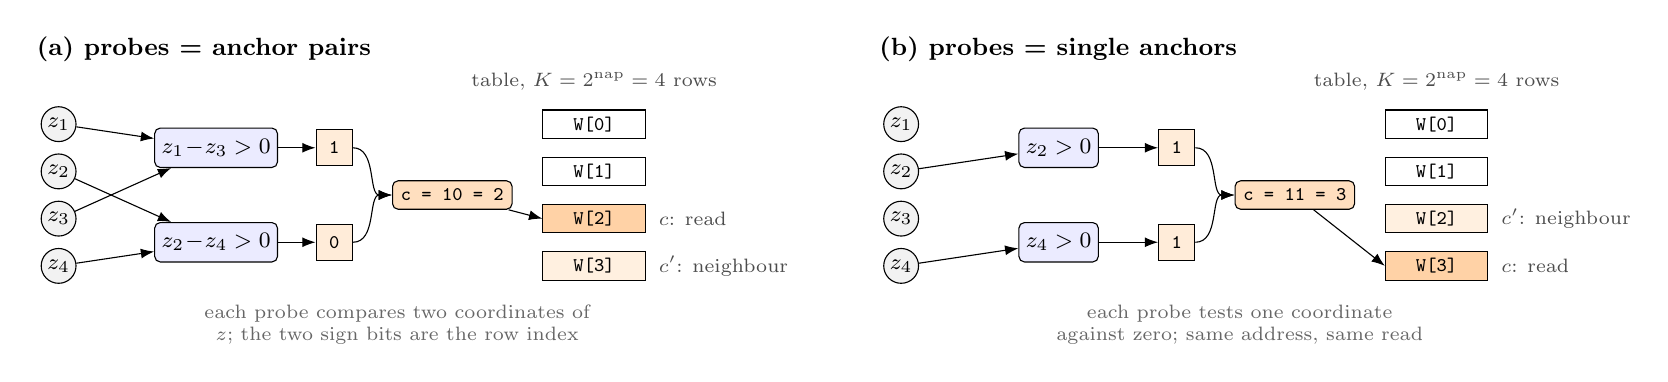
\begin{tikzpicture}[>=Latex, font=\footnotesize,
  coord/.style={draw, circle, inner sep=1.2pt, minimum size=4.4mm, fill=black!5},
  cmp/.style={draw, rounded corners=2pt, inner sep=2.5pt, minimum height=5mm, fill=blue!8},
  bit/.style={draw, inner sep=2pt, minimum size=4.6mm, fill=orange!15, font=\scriptsize\ttfamily},
  idx/.style={draw, rounded corners=2pt, fill=orange!25, inner sep=3pt, font=\scriptsize\ttfamily},
  row/.style={draw, minimum width=13mm, minimum height=3.6mm, inner sep=0pt, font=\scriptsize\ttfamily},
  tag/.style={font=\scriptsize, text=black!70},
  note/.style={font=\scriptsize, text=black!60, align=center, text width=58mm}]
% ================= panel (a): anchor pairs =================
\begin{scope}
\node[font=\small\bfseries, anchor=west] at (-0.4,2.75) {(a) probes = anchor pairs};
\foreach \i/\y in {1/1.8,2/1.2,3/0.6,4/0.0}{\node[coord] (z\i) at (0,\y) {$z_{\i}$};}
\node[cmp] (c1) at (2.0,1.5) {$z_1\!-\!z_3>0$};
\node[cmp] (c2) at (2.0,0.3) {$z_2\!-\!z_4>0$};
\draw[->] (z1) -- (c1); \draw[->] (z3) -- (c1);
\draw[->] (z2) -- (c2); \draw[->] (z4) -- (c2);
\node[bit] (b1) at (3.5,1.5) {1};
\node[bit] (b2) at (3.5,0.3) {0};
\draw[->] (c1) -- (b1); \draw[->] (c2) -- (b2);
\node[idx] (ix) at (5.0,0.9) {c = 10 = 2};
\draw[->] (b1.east) to[out=0,in=180] (ix.west);
\draw[->] (b2.east) to[out=0,in=180] (ix.west);
\foreach \r/\y in {0/1.8,1/1.2,2/0.6,3/0.0}{\node[row] (r\r) at (6.8,\y) {W[\r]};}
\node[row, fill=orange!35] (rc) at (6.8,0.6) {W[2]};
\node[row, fill=orange!12] (ra) at (6.8,0.0) {W[3]};
\node[tag, anchor=west] at (7.5,0.6) {$c$: read};
\node[tag, anchor=west] at (7.5,0.0) {$c'$: neighbour};
\node[tag, anchor=south] at (6.8,2.1) {table, $K=2^{\text{nap}}=4$ rows};
\draw[->] (ix) -- (rc.west);
\node[note] at (4.3,-0.75) {each probe compares two coordinates of $z$; the two sign bits are the row index};
\end{scope}
% ================= panel (b): single anchors =================
\begin{scope}[xshift=10.7cm]
\node[font=\small\bfseries, anchor=west] at (-0.4,2.75) {(b) probes = single anchors};
\foreach \i/\y in {1/1.8,2/1.2,3/0.6,4/0.0}{\node[coord] (s\i) at (0,\y) {$z_{\i}$};}
\node[cmp] (d1) at (2.0,1.5) {$z_2>0$};
\node[cmp] (d2) at (2.0,0.3) {$z_4>0$};
\draw[->] (s2) -- (d1);
\draw[->] (s4) -- (d2);
\node[bit] (e1) at (3.5,1.5) {1};
\node[bit] (e2) at (3.5,0.3) {1};
\draw[->] (d1) -- (e1); \draw[->] (d2) -- (e2);
\node[idx] (jx) at (5.0,0.9) {c = 11 = 3};
\draw[->] (e1.east) to[out=0,in=180] (jx.west);
\draw[->] (e2.east) to[out=0,in=180] (jx.west);
\foreach \r/\y in {0/1.8,1/1.2,2/0.6,3/0.0}{\node[row] (q\r) at (6.8,\y) {W[\r]};}
\node[row, fill=orange!35] (qc) at (6.8,0.0) {W[3]};
\node[row, fill=orange!12] (qa) at (6.8,0.6) {W[2]};
\node[tag, anchor=west] at (7.5,0.0) {$c$: read};
\node[tag, anchor=west] at (7.5,0.6) {$c'$: neighbour};
\node[tag, anchor=south] at (6.8,2.1) {table, $K=2^{\text{nap}}=4$ rows};
\draw[->] (jx) -- (qc.west);
\node[note] at (4.3,-0.75) {each probe tests one coordinate against zero; same address, same read};
\end{scope}
\end{tikzpicture}}
\caption{One lookup table in each of the two modes, \code{nap}$=2$. A probe yields one sign bit; the
bits, most significant first, form the row index $c$, which selects one learnable row of the
$K=2^{\text{nap}}$-row table. The probe with the smallest margin is the least certain, and flipping its
bit names the neighbour row $c'$ (lighter), which the richer read forms described later also fetch. (a) Anchor
pairs compare two coordinates of $z$; (b) single anchors test one coordinate against zero. A head sums
many such tables.}
\label{fig:table}
\end{figure}

% ======================================================================================================
\section{ProjectionLUT: input and output projections}
\label{sec:projection}

\code{ProjectionMHL} (the ``ProjectionLUT'' wrapper, Figure~\ref{fig:projlut}) puts a plain linear map on
each side of the cartridge --- the stack of tables together with its read mathematics --- so that, from
the outside, it takes an ordinary vector of width $D_\text{in}$ and returns one of width $D_\text{out}$,
like any feed-forward layer, while the tables work in their narrow per-head spaces. The two widths are
independent arguments of the wrapper and may differ. Writing $h_\text{in}$ and $h_\text{out}$ for the number of input and output heads and $d_\text{in}$,
$d_\text{out}$ for their widths ($h_\text{in}=h_\text{out}=G$ in the usual per-head case\footnote{The two head counts
may differ only when one of them is $1$; the library rejects every other combination. With
$h_\text{in}=1$ the input projection produces one $d_\text{in}$-wide slice that all $G$ heads read
(fan-out); with $h_\text{out}=1$ the heads' outputs are summed into one $d_\text{out}$-wide slice that
the output projection consumes (fan-in).}):
\[
  x\in[B,D_\text{in}]\ \xrightarrow{\ \code{compress}\ }\ z\in[B,h_\text{in},d_\text{in}]
  \ \xrightarrow{\ \code{cartridge}\ }\ y\in[B,h_\text{out},d_\text{out}]
  \ \xrightarrow{\ \code{decompress}\ }\ \text{out}\in[B,D_\text{out}].
\]
\begin{itemize}\itemsep1pt
\item \textbf{The input projection shapes the hashing.} A probe is also a hyperplane test, and what
  plane it tests depends on whether \code{compress} is in front and on the kind of probe:
  \begin{center}\footnotesize
  \begin{tabular}{@{}l >{\raggedright\arraybackslash}p{4.9cm} >{\raggedright\arraybackslash}p{5.6cm}@{}}
  \toprule
  & single anchors & anchor pairs \\
  \midrule
  \code{compress} off & $x[a]>0$: an axis-aligned plane of the raw input & $x[a]-x[b]>0$: coefficients $\pm1$, zero bias --- the manifesto's form \\
  \code{compress} on & $w_a^\top x+b_a>0$: an arbitrary learned hyperplane & $(w_a-w_b)^\top x+(b_a-b_b)>0$: also arbitrary; up to $\binom{d_\text{in}}{2}$ distinct planes per head \\
  \bottomrule
  \end{tabular}
  \end{center}
  With \code{compress} on, a single-anchor probe reads one row of the projection and is exactly the
  manifesto's ``hyperplane LSH'' with learnable anchor vectors (\citealp[\S VIII-H]{manifesto}).
  With \code{compress} in front, both modes get arbitrary hyperplanes, but the same projection yields far
  more distinct planes in pair form, so tables stop re-using the same few bits; single anchors are
  somewhat weaker, though not dramatically. Without \code{compress} the gap is large: a single anchor only
  tests the sign of one raw coordinate, an axis-aligned split, where a pair still compares two.
\item \textbf{The output projection compresses the tables.} A layer holds an exponential number of
  cells --- \code{tph} tables per head, $K=2^{\text{nap}}$ cells each, times the heads, so the count is
  exponential in \code{nap} --- and every cell stores a $d_\text{out}$-wide row, so the per-cell width
  $d_\text{out}$ is what controls table size. For example, with 8 heads of 64 tables
  and \code{nap}$=8$, that is $8\times64\times256=131{,}072$ cells per layer, $6.3$M table parameters at
  $d_\text{out}=48$; in a six-block model of width $384$ that is $37.7$M over six layers, more than half
  of its $68.2$M parameters, and at the full model width, $d_\text{out}=384$, it would be $50$M per layer. So the tables
  live in a narrow $d_\text{out}$, and
  \code{decompress} expands the concatenated head outputs back to model width afterwards, at the cost of one small
  dense map per layer ($0.15$M parameters).
\end{itemize}
Given a learned input projection, the single-anchor mode alone would have sufficed in principle: a pair
comparison $z[a]-z[b]>0$ is itself a hyperplane on $x$, so in principle anchor pairs could have been
dropped and the pair form left to \code{compress} to realise. In practice it would not be: ordinary
training has no reason to drive the \code{compress} matrix into a $\{+1,-1\}$ pair form, so recovering it
would take machinery this library does not have, such as strict regularisation or a straight-through
estimator onto $\pm1$ weights.

The library keeps both anchor modes deliberately. The pair comparison is the
Spiking Manifesto's mechanism as stated --- the relative order of two coordinates --- and it is the
cheap special case that the whole design is built to exploit: an address bit costs two coordinate reads
and one subtraction, with the anchors stored as integer indices and no weights of its own (the kernels
do exactly this), whereas a general per-table hyperplane would cost a $d_\text{in}$-length dot product and
$d_\text{in}$ weights per bit --- in the example above, with $d_\text{in}=48$, some 4{,}000 subtractions per token and layer
against about 200{,}000 multiply-adds. Single anchors were added later for flexibility, as the even
cheaper probe, and sit at the other end of the same trade.

Either projection --- the input projection \code{compress} or the output projection \code{decompress},
but not both --- may be switched off (Identity) when the widths already match. By default both are present, \code{decompress} is
initialised to zero and \code{compress} to $\mathcal{N}(0,0.02)$.

In code, the wrapper takes any cartridge --- the swappable read mathematics of \S\ref{sec:cartridges},
here \code{ConfidenceLUT} --- and maps $[N,D_\text{in}]$ to $[N,D_\text{out}]$, so a sequence is
flattened first:
\begin{lstlisting}
import torch
from spiky.lutorch_ex import LUTSpec, ConfidenceLUT, ProjectionMHL

spec = LUTSpec(h_in=8, h_out=8, tph=64, nap=8, d_in=48, d_out=48)  # 8 heads of 64 tables
cart = ConfidenceLUT(spec, seed=1, read_top_n=2)                    # the read mathematics
ffn  = ProjectionMHL(cart, d_model=384)          # or input_dim=..., output_dim=... (may differ)
x = torch.randn(4, 128, 384)                     # (B, T, D) activations
y = ffn(x.reshape(-1, 384)).reshape(x.shape)     # torch.Size([4, 128, 384])
\end{lstlisting}
Any other cartridge of \S\ref{sec:cartridges} can take \code{ConfidenceLUT}'s place.

\begin{figure}[t]
\centering
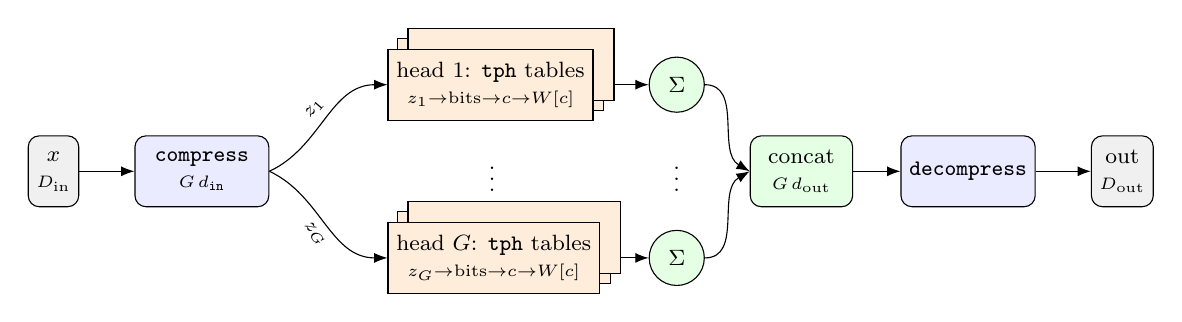
\begin{tikzpicture}[>=Latex, font=\footnotesize,
  box/.style={draw, rounded corners, align=center, inner sep=3pt, minimum height=9mm},
  io/.style={box, fill=black!6},
  proj/.style={box, fill=blue!8, minimum width=17mm, font=\footnotesize\ttfamily},
  tbl/.style={draw, fill=orange!14, align=center, inner sep=3pt, minimum width=24mm, minimum height=9mm},
  sumop/.style={draw, circle, inner sep=1pt, minimum size=7mm, fill=green!10}]
\node[io] (x) {$x$\\$\scriptstyle D_\text{in}$};
\node[proj, right=7mm of x] (cmp) {compress\\$\scriptstyle G\,d_\text{in}$};
\node[tbl, right=15mm of cmp, yshift=11mm] (t1) {head 1: \code{tph} tables\\$\scriptstyle z_1\to\text{bits}\to c\to W[c]$};
\node[tbl, right=15mm of cmp, yshift=-11mm] (t2) {head $G$: \code{tph} tables\\$\scriptstyle z_G\to\text{bits}\to c\to W[c]$};
\node at ($(t1)!0.5!(t2)$) {$\vdots$};
\node[sumop, right=7mm of t1] (s1) {$\Sigma$};
\node[sumop] (s2) at (s1 |- t2) {$\Sigma$};
\node at ($(s1)!0.5!(s2)$) {$\vdots$};
\node[box, fill=green!10, right=19mm of cmp, xshift=42mm, minimum width=13mm] (cat) {concat\\$\scriptstyle G\,d_\text{out}$};
\node[proj, right=6mm of cat] (dec) {decompress};
\node[io, right=7mm of dec] (y) {$\text{out}$\\$\scriptstyle D_\text{out}$};
\begin{scope}[on background layer]
  \foreach \t in {t1,t2}{ \foreach \dx in {1.3,2.6}{
    \draw[fill=orange!14, draw=black] ([xshift=\dx mm,yshift=\dx mm]\t.south east) rectangle ([xshift=\dx mm,yshift=\dx mm]\t.north west); }}
\end{scope}
\draw[->] (x) -- (cmp);
\draw[->] (cmp.east) to[out=25,in=180] node[above,sloped,font=\scriptsize]{$z_1$} (t1.west);
\draw[->] (cmp.east) to[out=-25,in=180] node[below,sloped,font=\scriptsize]{$z_G$} (t2.west);
\draw[->] ([xshift=2.6mm]t1.east) -- (s1);
\draw[->] ([xshift=2.6mm]t2.east) -- (s2);
\draw[->] (s1.east) to[out=0,in=150] (cat.west);
\draw[->] (s2.east) to[out=0,in=210] (cat.west);
\draw[->] (cat) -- (dec);
\draw[->] (dec) -- (y);
\end{tikzpicture}
\caption{The ProjectionLUT data path. The input projection \code{compress} ($D_\text{in}\to
h_\text{in}d_\text{in}$) splits $x$ into per-head spaces $z_g$; in each head the probes hash $z_g$ to a
cell per table and that head's \code{tph} reads are summed ($\Sigma$); the $G$ head outputs are
concatenated, and the output projection \code{decompress} ($h_\text{out}d_\text{out}\to D_\text{out}$)
maps the concatenation to the output. (With fan-in, $h_\text{out}=1$, the heads are summed into one slice
instead.) $D_\text{in}$ and $D_\text{out}$ are independent and may differ. The tables and per-head sums
are the cartridge; the wrapper treats it as opaque.}
\label{fig:projlut}
\end{figure}

% ======================================================================================================
\section{Cartridges}
\label{sec:cartridges}

Everything described so far is the same for every read form: the geometry, the addressing, the sum over
tables, the routing, the wrapper. A \emph{cartridge} is the swappable read \emph{mathematics} inside that
frame. The contract is a shape, $[B,h_\text{in},d_\text{in}]\to[B,h_\text{out},d_\text{out}]$
(\code{MultiHeadLUT}), and the wrapper never reaches inside it. All cartridges are built on one base class,
\code{ManifestoLUT}. It holds the tables $W\in\mathbb{R}^{G\times\text{tph}\times K\times d_\text{out}}$
and the anchors (drawn once from a seed, never trained), and it provides what every cartridge needs: the
addressed cell, the margins, the runner-up, and at the end the routing of each head's result to its output
slot. A cartridge decides the rest: how the addressed row and its neighbour are weighted and added up into
a head's output, and which function training differentiates. Gen-1 and Gen-2 also come as \code{Fused…}
twins with identical mathematics and faster kernels.

\subsection{One read, three ways to weight it}
\label{sec:oneread}
Every cartridge computes, per head,
\[
  y=\sum_t\big(a_t\,W_t[c_t]+b_t\,W_t[c_t']\big),
\]
with $c$ the addressed cell, $c'$ its least-certain-bit neighbour, and weights $a,b$ that depend on the
margins only. The generations differ in $a$ and $b$ (Table~\ref{tab:matrix}). The addresses are integers
and carry no gradient, so the input gradient flows through $a$ and $b$ alone.

\textbf{Hard and soft.} A \emph{soft} read uses the formula above as its value at train and eval, so both
rows learn. A \emph{hard} read returns $W[c]$ alone ($a=1$, $b=0$), adds rows without a multiply, and uses
the soft formula only as a \emph{surrogate} for the input gradient; the table update stays on row $c$.
Gen-1 and Gen-2 come in both forms. Gen-3 has no hard form: its weighted read is always the value.

\begin{table}[h]
\centering\footnotesize
\setlength{\tabcolsep}{4pt}
\begin{tabularx}{\textwidth}{@{}l l l >{\raggedright\arraybackslash}X@{}}
\toprule
generation & $a$, $b$ & learned scalars & cartridges (hard / soft) \\
\midrule
1 Manifesto (\S\ref{sec:manifesto}) & $1-U$, $U$ & --- & \code{ManifestoHardLUT} / \code{ManifestoSoftLUT} \\
2 SoftSign (\S\ref{sec:softsign}) & $1-w$, $w$ & $T_\text{soft},T_\text{sel}$ & \code{SoftSignHardLUT} / \code{SoftSignSmoothLUT} \\
3 Confidence (\S\ref{sec:confidence}) & $s(1-v)$, $s\,v$\ \ ($n{=}2$); $s$, $0$\ \ ($n{=}1$) & $\beta,\gamma$ (+$\tau$) & no hard form: \code{ConfidenceLUT}, int8 \code{QuantisedConfidenceLUT} (\S\ref{sec:quant}) \\
\bottomrule
\end{tabularx}
\caption{The three generations as weights on the addressed row and its neighbour. Gen-1 and Gen-2 each
also have \code{Fused…} twins of both forms.}
\label{tab:matrix}
\end{table}


\subsection{Gen-1 Manifesto}
\label{sec:manifesto}
The Spiking Manifesto's model~\citep{manifesto}, with the paper's fixed uncertainty function of the
deciding margin $|u_{j^\star}|=u^\star$:
\[
  U=\frac{0.5}{1+u^\star}\in(0,\tfrac12],\qquad
  \frac{\partial\tilde y}{\partial z[a_{j^\star}]}=-\frac{\partial\tilde y}{\partial z[b_{j^\star}]}
  =U'(u^\star)\,\sgn(u_{j^\star})\,\big(W[c']-W[c]\big),
\]
so the input gradient lands on the two anchors of the deciding probe alone (manifesto Eqs.~4--5).
\code{ManifestoHardLUT} is Izhikevich's rule verbatim: its value has $a=1$, $b=0$, and $a=1-U$, $b=U$
serve only as the surrogate. \code{ManifestoSoftLUT} promotes the surrogate Eq.~4 to the value, $a=1-U$,
$b=U$, which goes beyond the paper: there $U$ only computes training gradients, and inference reads
with Eq.~3 alone (manifesto \S III-A).

\subsection{Gen-2 SoftSign}
\label{sec:softsign}
The fixed $U$ becomes a blend weight with two temperatures learned per layer (init $0.5$, freezable):
\[
  \rho=\frac{u^\star}{T_\text{soft}+u^\star}\in[0,1),\qquad
  w=\sigma\!\big(-2\rho/T_\text{sel}\big)\in(0,\tfrac12].
\]
\code{SoftSignSmoothLUT} reads with $a=1-w$, $b=w$; \code{SoftSignHardLUT} reads $a=1$, $b=0$ and uses
$a=1-w$, $b=w$ as its surrogate.

\subsection{Gen-3 Confidence}
\label{sec:confidence}
Gen-3 weights each table by a \emph{confidence score} $s$, the score of LookupFFN~\citep{lookupffn},
computed from all \code{nap} margins $m_j=|u_j|$ of the table's address:
\[
  s=\Big(\sum_j m_j\Big)\exp\!\Big(\gamma\sum_j\log\sigma(\beta m_j)\Big),\qquad
  v=\sigma(-2u^\star/\tau)\in(0,\tfrac12].
\]
The sum of the margins grows with how far the input sits from the bit boundaries; the second factor is
the product of $\sigma(\beta m_j)^\gamma$ over the margins, near $1$ for a margin far from its boundary
and $2^{-\gamma}$ for a margin of zero, so every uncertain bit discounts the table. $\beta$ sets what
counts as a large margin, $\gamma$ how strong the discount is. $\beta$, $\gamma$ (and $\tau$) are learned scalars, one each per layer,
shared by all its tables and stored in log form (init $2,1,0.5$). With $n{=}1$ the scored cell is the whole read,
$a=s$, $b=0$, no blend. With $n{=}2$ the score multiplies a two-cell blend by uncertainty, as in Gen-2:
$a=s(1-v)$, $b=s\,v$, where the neighbour weight $v$ depends only on the deciding margin $u^\star$ and
$\tau$. The key property: the input
gradient reaches $z$ \emph{only} through $s$ (all \code{nap} margins) and, for $n{=}2$, through $v$ (the
deciding margin). A table learns how confident to be, never that a different row would have been better.

\subsection{The int8 read and deployment}
\label{sec:quant}
\textbf{Why.} The tables are most of a LUT model: in the example of \S\ref{sec:projection}, $6.3$M table
parameters per layer, $37.7$M of the model's $68.2$M. Stored as int8 instead of fp32 they take a quarter of
the memory. \code{QuantisedConfidenceLUT} (\code{quant\_mode="p2\_int8"}) is the
Gen-3 cartridge ($n{=}2$) trained for that deployed form.

\textbf{What p2\_int8 is.} Two roundings turn the read $s(1-v)\,W[c]+s\,v\,W[c']$ into integer work:
\begin{enumerate}\itemsep1pt
\item \textbf{int8 cells.} Each row is stored as $\hat W=\operatorname{clamp}(\operatorname{round}(W/2^{e}),-128,127)$,
  with one power-of-two scale per group and output channel, $e=\lceil\log_2\max|W|\rceil-7$ (the maximum over
  all of the group's tables and cells), so the largest entry just fits in eight bits.
\item \textbf{Power-of-two weights.} Write the read as $s(1-v)\,(W[c]+r\,W[c'])$ with
  $r=v/(1-v)=e^{-2u^\star/\tau}$. Round $r$ to $2^{-q}$, $q=\operatorname{round}\big(2u^\star/(\tau\ln2)\big)$,
  and $s(1-v)=s/(1+r)$ to $2^{k'}$, $k'=\operatorname{round}(\log_2 s-c_q)$ with $c_q=\log_2(1+2^{-q})$. A
  table then adds $2^{k'}\hat W[c]+2^{k'-q}\hat W[c']$: two shifts and an add, no multiply.
\item \textbf{Integer sum.} Shifts are counted in units of $2^{-6}$, so all are left shifts into an int32
  accumulator; the only float left is the per-channel $2^{e-6}$, applied once after the table sum.
\end{enumerate}
The exponents $q$ and $k'$ are computed from the margins in floating point; the table read itself is
integer. $q$ is capped at $64$ and $c_q$ taken as $0$ for $q\ge8$; $k'$ is kept in $[-3,4]$ (below,
the table is skipped but keeps its gradient; above, $k'$ is clamped); the neighbour cell is dropped when
$q>3$.

\textbf{Training is quant-aware.} The training forward already reads the rounded tables with the rounded
weights. Both roundings are straight-through:
the value is the rounded read, while the gradient is that of the float master tables and of the exact
weights $s(1-v)$, $s\,v$, so $\beta,\gamma,\tau$ keep learning.

\textbf{Deployment.} Because training is quant-aware, the deployed numbers are the trained numbers, up to
round-off: every training forward already computes with the int8 tables $\hat W$ and scales $2^e$ derived
from the float masters. Export is a change of storage, not of the model: \code{export\_deployment} stores those int8
values, drops the float masters, and bakes the scale $2^{e-6}$ \emph{statically} into a copy of the layer's
\code{decompress} weight --- exact, since a power of two changes only a float's exponent; no runtime hook
applies a scale afterwards. The file holds the int8 tables, the anchors and the three scalars: $24$~MiB $\to$ $6$~MiB per layer in the example. \code{load\_deployment} builds the model on
PyTorch's \code{meta} device and fills it from the file, so the float tables are never allocated. The
deployed layer returns the integer accumulator, and \code{decompress} applies the folded scale.
\begin{lstlisting}
export_deployment(model, "m.lxq")
dep = load_deployment("m.lxq", make_skeleton, device="cuda").eval()
\end{lstlisting}

\subsection{Which to use}
\label{sec:which}
For accuracy, \code{ConfidenceLUT} $n{=}2$. For deployment, its int8 twin \code{QuantisedConfidenceLUT}.
Gen-1 and Gen-2 are reference points; a hard read is the cheapest possible inference, at a cost in
accuracy against its soft twin.

% ======================================================================================================
\section{Regularisers}
\label{sec:reg}
Two regularisers live in the shared base class \code{ManifestoLUT}, so every cartridge has them; both
are off by default.

\paragraph{Cell total variation.} The $K=2^{\text{nap}}$ cells of a table are the corners of an
\code{nap}-dimensional cube: two cells are neighbours when their addresses differ in one bit, as $c$ and
$c'$ do. The penalty of a layer is the mean squared difference between neighbouring rows,
\[
  \mathcal R_\text{TV}=\frac{1}{T\cdot\text{nap}\cdot2^{\text{nap}-1}}
  \sum_{t=1}^{T}\ \sum_{(c,c')\,\text{Hamming-1}}\big\|W_t[c]-W_t[c']\big\|_2^2,
\]
over all $T=G\cdot\text{tph}$ tables and every neighbouring pair, each counted once
(\code{ManifestoLUT.cell\_tv}). \code{cell\_tv\_penalty(model)} averages it over the model's LUT layers,
and the training loss adds $\lambda$ times that. It acts on the table weights only and leaves the forward
pass unchanged. The prior it encodes: a one-bit change of address, the smallest change of input, should
change the read only a little.

\paragraph{Table dropout.} With \code{table\_dropout\_rate} $p>0$, training drops whole tables: one
Bernoulli draw per sample, head and table keeps each table with probability $1-p$, and the survivors
are scaled by $1/(1-p)$, so the expected read is unchanged. A dropped table contributes nothing to that
sample's value or gradient; in Gen-3 the mask multiplies the score $s$, to the same effect. At evaluation,
or whenever gradients are off, nothing is dropped and nothing is rescaled.

% ======================================================================================================
\section{Experiments: the seven-configuration sweep}
\label{sec:ml}
\suppressfloats[t]% keep the results table from floating above this heading

\paragraph{Setup.} A six-block GPT ($d_\text{model}=384$, 6 attention heads, $68.2$M parameters) with the
feed-forward layer of every block replaced by a \code{ProjectionMHL} around the cartridge under test.
Every configuration here is square: the wrapper's input and output widths both equal the model width,
$D_\text{in}=D_\text{out}=d_\text{model}=384$. All
seven runs\footnote{Configs, full metric histories and summaries (including wall-clock hours and peak
memory) of every run are on the branch, under
\url{https://github.com/anatoli-starostin/spiky/tree/feature/lutorch_ex_report/experiments/lutorch_ex}.}
share the same topology --- $h_\text{in}=h_\text{out}=8$, \code{tph}$=64$, \code{nap}$=8$,
$d_\text{in}=d_\text{out}=48$, anchor pairs --- seed~1, the default init (per-head Uniform$[\pm10^{-3}]$
tables, \code{decompress} zeroed), cell TV $\lambda=10$ and table dropout $p=0.2$ (\S\ref{sec:reg}), AdamW ($3\!\times\!10^{-4}$, weight decay $0.1$, none on the tables),
48{,}000 steps, cosine schedule with $10\%$ warm-up to a $0.1\times$ floor, sequence length 512, 24{,}576
tokens per step (device batch 12, accumulation 4), evaluation every 500 steps; the backbone runs in bf16,
the LUT layers in fp32. Data and tokenisation are the \emph{NanoChat} setup: the ClimbMix text corpus as
prepared by nanochat's data script, streamed and tokenised on the fly by nanochat's RustBPE tokenizer
(32{,}768-entry vocabulary, trained by nanochat on the same corpus) into BOS-aligned 512-token rows;
\code{val\_bpb} is the validation cross-entropy in bits divided by the number of \emph{bytes} of the
decoded text (nanochat's bits-per-byte evaluation on a fixed held-out set), so it is comparable across
tokenisers.

\begin{table}[t]
\centering\footnotesize
\setlength{\tabcolsep}{4pt}
\begin{tabular}{@{}l l r r r@{}}
\toprule
feed-forward layer & read & params & best \code{val\_bpb} & $\Delta$ vs.\ dense \\
\midrule
dense FFN, $384\!\to\!1536\!\to\!384$, GELU & --- & 35.8M & 1.11509 & --- \\
\midrule
\code{ConfidenceLUT} $n{=}2$        & scored two-cell blend, float   & 68.2M & \textbf{1.10606} & $-0.0090$ \\
\code{QuantisedConfidenceLUT} $n{=}2$ & the same, int8 + power-of-two & 68.2M & 1.10724 & $-0.0079$ \\
\code{ConfidenceLUT} $n{=}1$        & scored single cell             & 68.2M & 1.11737 & $+0.0023$ \\
\code{FusedSoftSignSmoothLUT}       & learned-temperature blend      & 68.2M & 1.12941 & $+0.0143$ \\
\code{FusedManifestoSoftLUT}        & $U$-blend                      & 68.2M & 1.13949 & $+0.0244$ \\
\code{FusedManifestoHardLUT}        & hard read                      & 68.2M & 1.15152 & $+0.0364$ \\
\code{FusedSoftSignHardLUT}         & hard read                      & 68.2M & 1.15647 & $+0.0414$ \\
\bottomrule
\end{tabular}
\caption{The 48k sweep, one seed, against the dense feed-forward baseline: the same backbone (6 blocks,
$d_\text{model}=384$, 6 attention heads), data, tokenizer, schedule, 24{,}576-token batches and seed, with
the dense $384\!\to\!1536\!\to\!384$ GELU layer in the feed-forward slot (run
\code{exp\_n\_0177\_vanilla48k\_corrected} on branch \code{research/ffn\_replacement\_fix}).}
\label{tab:results}
\end{table}

\begin{figure}[t]
\centering
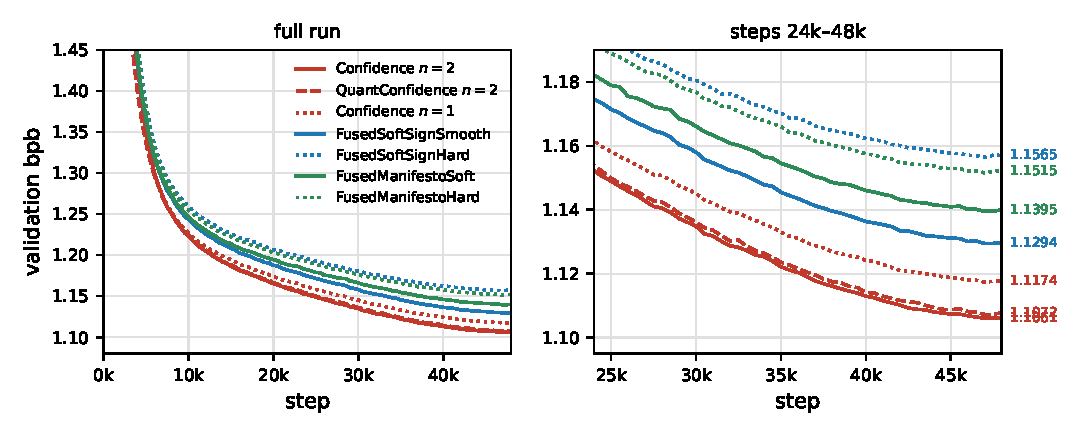
\includegraphics[width=\linewidth]{fig_curves.pdf}
\caption{Validation bpb of the seven runs (left: full run; right: the last half, with each run's best value).
Colour is the generation (red Confidence, blue SoftSign, green Manifesto); dotted lines are the
one-cell reads (the two hard reads and Confidence $n{=}1$), dashed is the int8 cartridge.}
\label{fig:curves}
\end{figure}

\paragraph{Reading the results.} Five things are visible in Table~\ref{tab:results} and
Figure~\ref{fig:curves}; each is one run per configuration. (i) In the two generations that come in a
hard and a soft form, the \emph{soft} read is better: by $0.012$ bpb for Manifesto and $0.027$ for
SoftSign. (ii) Within Gen-3, also reading the neighbour cell ($n{=}2$) beats the single scored cell
($n{=}1$) by $0.011$. Both are soft, scored reads, so this compares one cell with two, not hard with soft.
(iii) Adding the \emph{confidence score} beats a blend by uncertainty alone: Confidence $n{=}2$ leads the
best SoftSign run by $0.023$ and the best Manifesto run by $0.033$. The order of all seven runs is fixed
from step 7{,}500 on. (iv) \emph{Quantisation is nearly free}: int8 rows and power-of-two weights cost $+0.0012$ bpb,
for tables one quarter the size. (v) Against the
dense feed-forward layer, the two scored two-cell cartridges \emph{win} ($-0.009$ and $-0.008$ bpb), the
single-cell scored read is within $0.002$, and the blend-only generations trail by $0.014$--$0.041$; the
LUT models carry $1.9\times$ the parameters of the dense one, but a LUT layer touches only two 48-wide rows
per table per token.

\subsection{Benchmarks: CPU, RTX 5090, H100}
\label{sec:bench}
Table~\ref{tab:bench} times the layer alone, at the sweep geometry, for the seven optimised configurations
the sweep used: the four fused twins and the three Gen-3 configurations (which have no separate twin:
their \code{embedding\_bag} read with a compiled forward is already the fast path). Gen-1 and Gen-2 also
exist as plain-PyTorch \emph{reference} cartridges (\code{ManifestoHardLUT} and so on): written for
readability, and the oracle the fused twins are tested against for equal results. They are not tuned for
speed and the sweep did not train with them, so the table leaves them out. The CPU and RTX 5090 columns
were measured for this report with the library's benchmark harness, the module
\code{spiky.lutorch\_ex.bench} (\code{src/spiky/lutorch\_ex/bench.py}), driven by the script
\code{bench\_report.py}. That script and its per-cell output are on the branch named in the footnote of
\S\ref{sec:ml}, under \code{doc/research/lutorch\_ex\_report/}; the run results are under
\code{experiments/lutorch\_ex/} on the same branch.

\begin{table}[h]
\centering\footnotesize
\setlength{\tabcolsep}{3.6pt}
\begin{tabular}{@{}l r rrr rrr@{}}
\toprule
& CPU (measured) & \multicolumn{3}{c}{RTX 5090 (measured)} & \multicolumn{3}{c}{H100 (recorded, PR \#138)} \\
\cmidrule(lr){2-2}\cmidrule(lr){3-5}\cmidrule(l){6-8}
cartridge & step ms, $B{=}1024$ & eval ms & step ms & peak GB & eval ms & step ms & peak GB \\
\midrule
\code{FusedManifestoHardLUT}        & 62.9 & 1.04 & 20.2 & 3.8 & 1.61 & 21.3 & 4.0 \\
\code{FusedManifestoSoftLUT}        & 92.3 & 3.50 & 22.5 & 2.3 & 3.84 & 23.6 & 2.5 \\
\code{FusedSoftSignHardLUT}         & 68.8 & 1.03 & 24.6 & 4.2 & 1.61 & 23.8 & 4.2 \\
\code{FusedSoftSignSmoothLUT}       & 60.8 & 2.13 & 28.8 & 2.9 & 4.10 & 28.4 & 3.0 \\
\code{ConfidenceLUT} $n{=}1$        & 35.8 & 1.51 & 11.5 & 1.1 & 2.40 & 12.9 & 1.2 \\
\code{ConfidenceLUT} $n{=}2$        & 66.7 & 4.59 & 21.5 & 1.9 & 4.17 & 24.7 & 2.1 \\
\code{QuantisedConfidenceLUT} $n{=}2$ & 83.4 & 4.12 & 23.9 & 1.8 & 4.23 & 24.5 & 2.0 \\
\bottomrule
\end{tabular}
\caption{Layer-only timings at $h_\text{in}=h_\text{out}=8$, \code{tph}$=64$, \code{nap}$=8$,
$d_\text{in}=d_\text{out}=48$, fp32, random input. \emph{eval} = no-grad forward; \emph{step} = training
forward + backward. GPU columns at $B=24{,}576$ (the sweep's training batch). \textbf{Measured here:}
one workstation, torch 2.9.1 (cu130), CUDA 13.3 toolkit for the JIT kernels, driver 595; RTX 5090 (32\,GB,
native kernels active): medians of 10 repeats after 3 warm-ups; CPU (24-thread desktop part, the fused
twins' \code{embedding\_bag} path, $B=1{,}024$): medians of 15 repeats after 5 warm-ups, with the
fastest repeat within $15\%$ of the median (\code{bench\_cpu.json} and
\code{bench\_cuda.json} beside that script hold every cell). H100 column measured on an H100 VM provided by Nebius.}
\label{tab:bench}
\end{table}

Three readings. On either GPU the training step of every blend or hard cartridge is $20$--$29$ ms at the
training batch and is dominated by the backward ($17$--$19$ ms), the scatter into the $6.3$M-entry table;
\code{ConfidenceLUT} $n{=}1$ is both the cheapest step ($11.5$ ms) and the smallest footprint ($1.1$
GB), because its compiled forward fuses the score's chain of small kernels and reads one cell. Reading two
cells ($n{=}2$, the soft forms) roughly doubles the eval forward ($1.0\to3.5$ ms for Manifesto,
$1.5\to4.6$ ms for Confidence). The quantised cartridge's eval forward is not faster than the float one
--- its training-time read still fetches float rows for the straight-through estimator; the integer read
belongs to the deployed cartridge (\S\ref{sec:quant}). The fused twins earn their place:
\code{FusedSoftSignHardLUT}'s native training step is $1.6\times$ faster and uses $2.7\times$ less memory
than its reference cartridge \code{SoftSignHardLUT} at the training batch (recorded when the twin landed;
the reference cartridges are not in Table~\ref{tab:bench}). The two GPUs agree to within $15\%$ on every row:
these layers are bound by memory traffic, not arithmetic. On the CPU, at a batch $24\times$ smaller, the
same layers take $36$--$92$ ms per step --- roughly two orders of magnitude slower per row --- with the
same ordering: the one-cell scored read is the cheapest, the two-cell blends cost $1.7$--$2.6\times$ more.

\begin{thebibliography}{9}\small
\bibitem{manifesto} E.~M.~Izhikevich. ``Spiking Manifesto.'' arXiv:2512.11843, v2, December 2025.
\bibitem{lookupffn} Z.~Zeng, M.~Davies, P.~Pulijala, K.~Sankaralingam, V.~Singh. ``LookupFFN: Making
  Transformers Compute-lite for CPU Inference.'' ICML 2024.
\end{thebibliography}

\end{document}
